\section{ĐỀ SỐ \thesection }%ĐỀ 5
\setcounter{bt}{0}

%%Câu 1.
\begin{bt} \textbf{ }
	\begin{listEX}
		\item Sắp xếp các số nguyên sau theo thứ tự giảm dần: $-16 ;\ 95 ;\ -22 ;\ 23$
		\item Biểu diễn các số nguyên sau trên trục số: $3 ;\ -4 ;\ 0 ;\ -6$.
		\item Tìm số nguyên $x$, biết $x+194=-25$.
	\end{listEX}
	
	\loigiai{a) $95, 23, -16, -22$ \hfill b) Học sinh tự biểu diễn \hfill c) $x = -219$}
\end{bt}

%%Câu 2.
\begin{bt} \textbf{ }
	\begin{listEX}
		\item Vẽ hình bình hành $ABCD$ có $AB=3$ cm, $BC=5$ cm.
		\item Tính chu vi và diện tích hình thoi $MNPQ$ có $MN=20$ cm, $ PM=32$ cm, $NQ=24$ cm.
	\end{listEX}
	\loigiai{a) Học sinh tự vẽ hình \hfill b) $80 \text{ cm}; 384 \text{ cm}^2$}
\end{bt}


%%Câu 3.
\begin{bt} Điều tra về điểm một bài kiểm tra thường xuyên môn Toán của 36 học sinh lớp 6B, bạn lớp trưởng thu được bảng dữ liệu sau :
	
	\begin{center}
		\begin{tabular}{|c|c|c|c|c|c|c|c|c|c|c|c|}
			\hline
			10 & 9 & 3 & 6 & 5 & 8 & 10 & 9 & 7 & 6 & 9 & 7 \\
			\hline
			8 & 10 & 6 & 10 & 10 & 4 & 6 & 5 & 10 & 9 & 4 & 7 \\
			\hline
			8 & 9 & 5 & 9 & 8 & 6 & 9 & 7 & 6 & 7 & 5 & 9 \\
			\hline
		\end{tabular}
	\end{center}
	\begin{listEX}
		\item Hãy gọi tên bảng dữ liệu ở trên.
		\item Hãy lập bảng thống kê tương ứng và cho biết điểm số nào có số học sinh đạt được nhiều nhất.
	\end{listEX}	
	\loigiai{\begin{listEX} 
			\item Bảng điều tra điểm kiểm tra thường xuyên môn Toán của lớp 6B 
			\item Điểm số đạt được nhiều nhất là 9, mỗi điểm có 8 học sinh
		\end{listEX}}
	
\end{bt}


%%Câu 4.
\begin{bt} Tìm $\operatorname{BCNN}(60 ; 75 ; 150)$ rồi quy đồng mẫu các phân số $\frac{7}{60} ;\  \frac{11}{75}$ và $\frac{13}{150}$.
	
	\loigiai{$\operatorname{BCNN}(60, 75, 150) = 300$; các phân số sau khi quy đồng là $\frac{35}{300}, \frac{44}{300}, \frac{26}{300}$}
\end{bt}

%%Câu 5.
\begin{bt} \textbf{ }
	\begin{listEX}
		\item Bỏ dấu ngoặc rồi tính bằng cách hợp lí: $-(-123+456-789)+(-123+3456-6789)$.
		\item Một tàu ngầm trên mặt đại dương lặn xuống với tốc độ $2$ m/s trong $2$ phút. Sau đó, nó nổi lên với tốc độ $1$ m/s trong $3$ phút. Lúc này, độ cao của tàu ngầm so với bề mặt đại dương là bao nhiêu?
	\end{listEX}
	\loigiai{a) $-3000$ \hfill b) $-60$
	}
\end{bt}


%%Câu 6.
\begin{bt} Tính diện tích phần được tô đậm trong hình vẽ dưới đây (biển báo hình vuông, chiều cao mũi tên là 35 cm)
	\begin{center}
		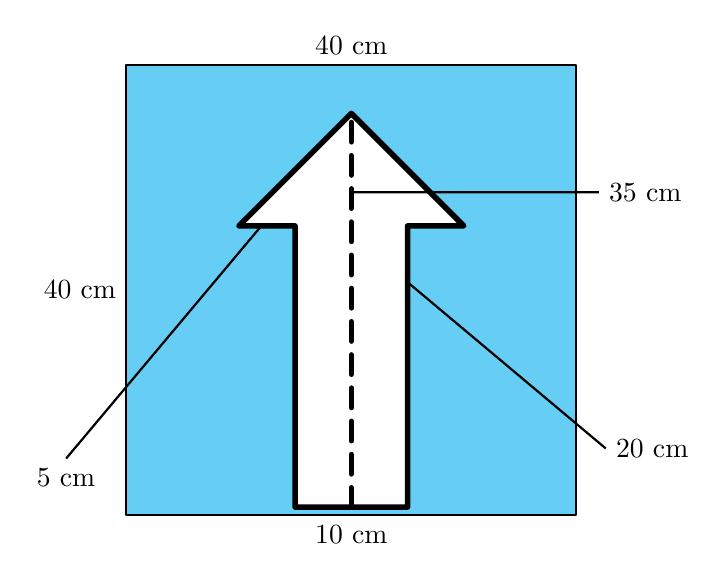
\begin{tikzpicture}[scale=1,line width=0.8pt,line join=round,>=stealth]
			\def\a{7}
			\path (0,0) coordinate (A)
			(0,35/\a) coordinate (B)
			;
			\draw[fill=cyan!60] (-20/\a,-0.1) -- (-20/\a,40/\a-0.1)node[midway,left]{40 cm} -- (20/\a,40/\a-0.1)node[midway,above]{40 cm}--(20/\a,-0.1)-- cycle node[midway,below]{10 cm};
			\draw[fill=white,line width=2pt] (0,35/\a)--++(10/\a,-10/\a)--++(180:5/\a)--++(-90:25/\a)--++(180:10/\a)--++(90:25/\a)--++(180:5/\a)--cycle;
			\draw[dash pattern=on 7pt off 5pt,line width=2pt,line cap=round] (0,0)--(90:35/\a);
			\draw[thick] (0,28/\a)--++(0:22/\a)node[right]{35 cm}
			(-8/\a,25/\a)--++(-130:27/\a)node[below]{5 cm}
			(5/\a,20/\a)--++(-40:23/\a)node[right] {20 cm};
		\end{tikzpicture}
	\end{center}
	\loigiai{$1250$ $m^2$}
\end{bt}


